\documentclass[margin=2cm]{standalone}

\usepackage[dvipsnames]{xcolor}
\usepackage{tikz}
\usetikzlibrary{positioning, calc}

\begin{document}
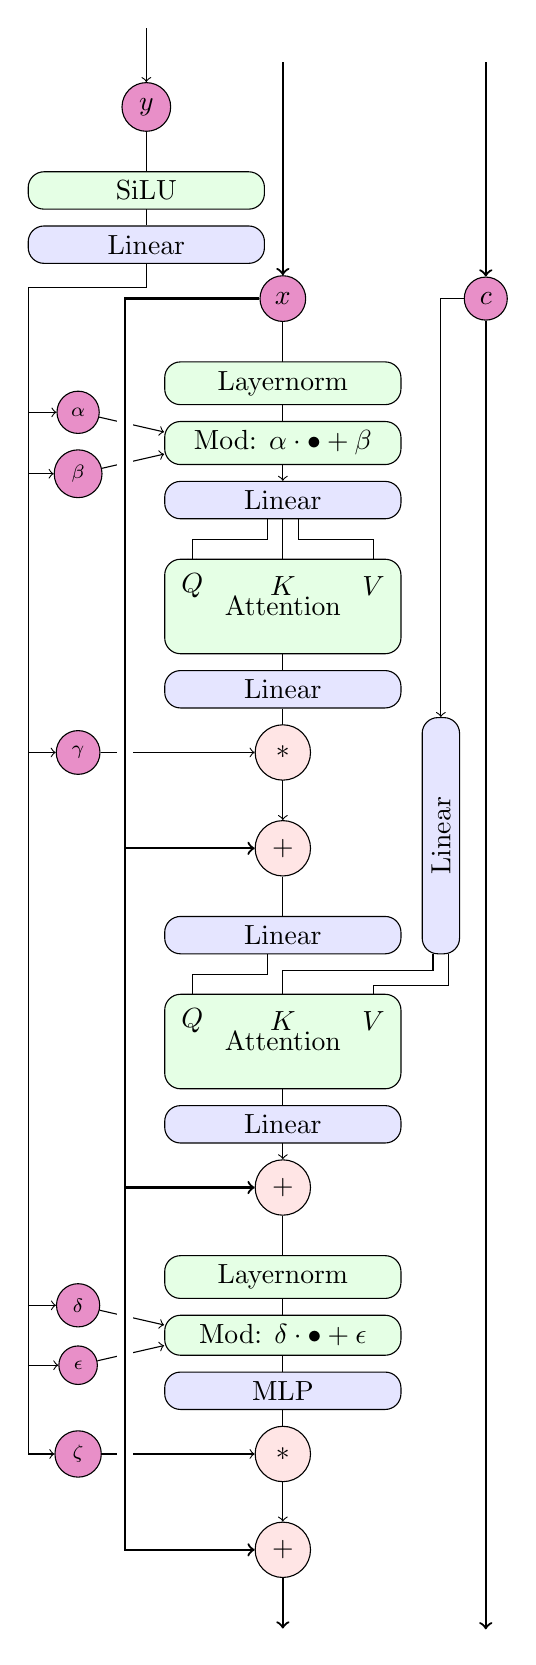
\begin{tikzpicture}[
        block/.style={draw, fill=white, rectangle, minimum width=3cm, rounded corners=0.2cm},
        trainableblock/.style={block,fill=blue!10},
        fnblock/.style={block,fill=green!10},
        operation/.style={draw, fill=red!10, circle, minimum width=2em},
        tensor/.style={draw, fill=VioletRed!50, circle},
    ]
    \pgfdeclarelayer{arrowlayer}
    \pgfdeclarelayer{residuallayer}
    \pgfsetlayers{arrowlayer,residuallayer,main}
    
    \newcommand{\inblockdistance}{0.2cm}
    \newcommand{\outblockdistance}{0.5cm}
    \newcommand{\leftmodpos}{-2.6}
    \newcommand{\rightmodpos}{7.2}

    \node [tensor] (c) {$x$};
    \node [below=\outblockdistance of c, fnblock] (c_ln1) {Layernorm};
    \node [below=\inblockdistance of c_ln1, fnblock] (c_mod) {Mod: $\alpha \cdot \bullet + \beta$};
    \node [below=\inblockdistance of c_mod, trainableblock] (c_lin) {Linear};

    \node [fnblock, below=0.5cm of c_lin, minimum width=3cm, minimum height=1.2cm] (attn) {Attention};
    \node [below=\inblockdistance of attn, trainableblock] (c_proj) {Linear};

    \node [below=\inblockdistance of c_proj, operation] (c_proj_gated) {$*$};
    \node [below=\outblockdistance of c_proj_gated, operation] (c_attn_out) {$+$};

    \node [below=\outblockdistance of c_attn_out, trainableblock] (cross_attn_lin_x) {Linear};
    \node [below=0.5cm of cross_attn_lin_x, fnblock, minimum width=3cm, minimum height=1.2cm] (cross_attn) {Attention};
    \node [below=\inblockdistance of cross_attn, trainableblock] (cross_attn_proj) {Linear};
    \node [below=\inblockdistance of cross_attn_proj, operation] (cross_attn_plus) {$+$};

    \node [right=0.5cm of cross_attn_lin_x.south east, trainableblock, rotate=90, anchor=west] (cross_attn_lin_c) {Linear};

    \node [below=\outblockdistance of cross_attn_plus, fnblock] (c_ln2) {Layernorm};
    \node [below=\inblockdistance of c_ln2, fnblock] (c_mod2) {Mod: $\delta \cdot \bullet + \epsilon$};
    \node [below=\inblockdistance of c_mod2, trainableblock] (c_mlp) {MLP};
    \node [below=\inblockdistance of c_mlp, operation] (c_mlp_gated) {$*$};
    \node [below=\outblockdistance of c_mlp_gated, operation] (c_out) {$+$};

    \path let \p1=($(c_mod.north west)!0.5!(c_mod.west)+(0, 0.25)$) in node [tensor] at (\leftmodpos, \y1) (alpha_c) {$\scriptstyle \alpha$};
    \path let \p1=($(c_mod.south west)!0.5!(c_mod.west)-(0, 0.25)$) in node [tensor] at (\leftmodpos, \y1) (beta_c) {$\scriptstyle \beta$};
    \path let \p1=(c_proj_gated.west) in node [tensor] at (\leftmodpos, \y1) (gamma_c) {$\scriptstyle \gamma$};
    \path let \p1=($(c_mod2.north west)!0.5!(c_mod2.west)+(0, 0.25)$) in node [tensor] at (\leftmodpos, \y1) (delta_c) {$\scriptstyle \delta$};
    \path let \p1=($(c_mod2.south west)!0.5!(c_mod2.west)-(0, 0.25)$) in node [tensor] at (\leftmodpos, \y1) (epsilon_c) {$\scriptstyle \epsilon$};
    \path let \p1=(c_mlp_gated.west) in node [tensor] at (\leftmodpos, \y1) (zeta_c) {$\scriptstyle \zeta$};

    \node [tensor, above left=2cm and 1.3cm of c] (y) {$y$};
    \node [fnblock, below=\outblockdistance of y] (y_silu) {$\mathrm{SiLU}$};
    \node [trainableblock, below=\inblockdistance of y_silu] (y_linear) {Linear};
    \coordinate (y_split) at ($(y_linear.south)+(-1.5, -0.3)$);
    % \node [operation, below=\outblockdistance of y_linear] (y_split) {$:$};

    \coordinate (c_attn_out_left) at ($(c_attn_out) + (-2, 0)$);
    \coordinate (cross_attn_out_left) at ($(cross_attn_plus) + (-2, 0)$);

    \begin{pgfonlayer}{arrowlayer}
        \draw [->] (c) -- (c_lin);
        \draw [->] (attn) -- (c_proj) -- (c_attn_out);
        \draw [->] (cross_attn_plus) -- (c_out);

        % modulation
        \draw [<-] (y) --++ (0, 1);
        \draw (y) -- (y_linear) |- (y_split);
        \draw [->] (y_split) |- (alpha_c);
        \draw [->] (y_split) |- (beta_c);
        \draw [->] (y_split) |- (gamma_c);
        \draw [->] (y_split) |- (delta_c);
        \draw [->] (y_split) |- (epsilon_c);
        \draw [->] (y_split) |- (zeta_c);

        \draw [->] (alpha_c) -- ($(c_mod.north west)!0.5!(c_mod.west)$);
        \draw [->] (beta_c) -- ($(c_mod.south west)!0.5!(c_mod.west)$);
        \draw [->] (gamma_c) -- (c_proj_gated.west);
        \draw [->] (delta_c) -- ($(c_mod2.north west)!0.5!(c_mod2.west)$);
        \draw [->] (epsilon_c) -- ($(c_mod2.south west)!0.5!(c_mod2.west)$);
        \draw [->] (zeta_c) -- (c_mlp_gated.west);

        \draw (c_attn_out) -- (cross_attn_lin_x);
        \draw [->] (cross_attn) -- (cross_attn_plus);

    \end{pgfonlayer}
    \begin{pgfonlayer}{residuallayer}
        % residual connections
        \draw [<-, line width=2mm, draw=white] (c) --++ (0, 3);
        \draw [->, line width=2mm, draw=white] (c) -| (c_attn_out_left) -- (c_attn_out);
        \draw [->, line width=2mm, draw=white] (c_attn_out_left) |- (c_out);
        \draw [->, line width=2mm, draw=white] (c_out) --++ (0, -1);
        \draw [<-, thick] (c) --++ (0, 3);
        \draw [->, thick] (c) -| (c_attn_out_left) -- (c_attn_out);
        \draw [->, thick] (c_attn_out_left) |- (c_out);
        \draw [->, thick] (cross_attn_out_left) -- (cross_attn_plus);
        \draw [->, thick] (c_out) --++ (0, -1);

    \end{pgfonlayer}



    \node [below=0.1cm of attn.north] (k) {$K$};
    \node [left=0.6cm of k] (q) {$Q$};
    \node [right=0.6cm of k] (v) {$V$};
    \begin{pgfonlayer}{arrowlayer}
        \draw [->] ($(c_lin)-(0.2, 0)$) --++ (0, -0.5) -| (q);
        \draw [->] (c_lin) |- (k);
        \draw [->] ($(c_lin)+(0.2, 0)$) --++ (0, -0.5) -| (v);
    \end{pgfonlayer}


    \node [below=0.1cm of cross_attn.north] (k) {$K$};
    \node [left=0.6cm of k] (q) {$Q$};
    \node [right=0.6cm of k] (v) {$V$};
    \begin{pgfonlayer}{arrowlayer}
        \draw [->] ($(cross_attn_lin_x)-(0.2, 0)$) --++ (0, -0.5) -| (q);
        \draw [->] ($(cross_attn_lin_c.west)-(0.1, 0)$) --++ (0, -0.2) -| (k);
        \draw [->] ($(cross_attn_lin_c.west)+(0.1, 0)$) --++ (0, -0.4) -| (v);
    \end{pgfonlayer}

    \node [right=2cm of c, tensor] (real_c) {$c$};
    \begin{pgfonlayer}{arrowlayer}
        \draw [->] (real_c) -| (cross_attn_lin_c);
    \end{pgfonlayer}

    \begin{pgfonlayer}{residuallayer}
        \draw [<-, thick] (real_c) --++ (0, 3);
        \draw [->, thick] (real_c) --++ (0, -16.9);
    \end{pgfonlayer}
\end{tikzpicture}
\end{document}
